\section{Теоретические основы}

Метрическое пространство~---~это пара $ \left( S, d \right) $,
состоящая из множества $S$ и метрики $d \; : \; S \times S \rightarrow \mathbb{R}$,
то есть для любых $x, y, z \in S$ выполняется
\begin{enumerate}
  \item $d \left( x, y \right) \geq 0$;
  \item $d \left( x, y \right) = 0 \Longleftrightarrow x = y$~---~аксиома тождества;
  \item $d \left( x, y \right) = d \left( y, x \right) $~---~аксиома симметрии;
  \item $d \left( x, z \right) \leq d \left( x, y \right) + d \left( y, z \right) $ ---
  неравенство треугольника.
\end{enumerate}

Метрическое пространство $ \left( S, d \right) $ называется сепарабельным,
если существует не более чем счётное множество $ \Gamma \subset S$ такое, что
\begin{equation*}
  \left( \forall x \in S \right) \,
  \left( \forall \varepsilon > 0 \right) \,
  \left( \exists y \in \Gamma \right) \, : \qquad
  d \left( x, y \right) < \varepsilon.
\end{equation*}

Метрическое пространство $ \left( S, d \right) $ называется полным,
если в нём любая фундаментальная последовательность сходится.
Примером полного сепарабельного метрического пространства есть $ \mathbb{R}^n$
с евклидовым расстоянием.

\section{Расстояние Хаусдорфа}

Расстояние Хаусдорфа определяется на множестве
всех непустых замкнутых подмножеств пространства $ \mathbb{R}^n$.

Пусть $E$ и $F$~---~непустые замкнутые подмножества $ \mathbb{R}^n$.
Расстояние Хаусдорфа между $E$ и $F$ определяется как
\begin{equation}\label{eq:hausdorff:distance}
  H \left( E, F \right) =
  \inf \left\{ \varepsilon \geq 0 \; | \; E \subset F + \varepsilon, \, F = E + \varepsilon \right\},
\end{equation}
где $E + \varepsilon $~---~объединение замкнутых шаров
с радиусом $ \varepsilon $ и центром в точке $x \in E$
\begin{equation*}\label{eq:set:expansion}
  E + \varepsilon =
  \bigcup \limits_{x \in E} \left\{ \overline{B}_{ \varepsilon } \left( x \right) \right\}.
\end{equation*}

Проверим асиомы метрики для расстояния Хаусдорфа $H \left( E, F \right) $,
заданного формулой \eqref{eq:hausdorff:distance}.

\begin{enumerate}
  \item $H \left( E, F \right) \geq 0$.
  Это следует из определения \eqref{eq:hausdorff:distance},
  так как точная нижняя грань величины $ \varepsilon \geq 0$ неотрицательна.
  \item $H \left( E, F \right) = 0$ тогда и только тогда, когда $E = F$.
  Последнее равенство равносильно двум условиям: $E \subset F$ и $F \subset E$.
  Это можно записать через элементы множеств:
  если $x \in E$, то $x \in F$, и если $x \in F$, то $x \in E$.

  Пусть $x \in E$ и $ \forall \varepsilon > 0$ выполняется $F + \varepsilon \supset E$,
  то есть $x \in F + \varepsilon $.
  Воспользуемся определением \eqref{eq:set:expansion}
  $$x \in
    \bigcup \limits_{y \in F} \overline{B}_{ \varepsilon } \left( y \right).$$
  Если $x$ принадлежит объединению множеств, то он принадлежит хотя бы одному из этих множеств.
  Значит, найдётся такой $y_{ \varepsilon } \in F$,
  что $x \in \overline{B}_{ \varepsilon } \left( y_{ \varepsilon } \right) $,
  то есть $d \left( y_{ \varepsilon }, x \right) \leq \varepsilon $.
  Это выполнено при любом $ \varepsilon \geq 0$, следовательно,
  $x$ либо лежит в $F$, либо является его предельной точкой.
  Но $F$ --- замкнутое множество, откуда следует, что $x \in F$.

  Вторая часть доказывается аналогично.

  С другой стороны, если $E = F$, то $E \subset F$ и $F \subset E$,
  значит $ \varepsilon = 0$ и $H \left( E, F \right) = 0$.
  \item $H \left( E, F \right) = H \left( F, E \right) $
  следует из симметричности определения расстояния Хаусдорфа.
  \item $H \left( E, F \right) \leq H \left( E, F \right) + H \left( F, G \right) $
  для любых замкнутых множеств $E, F, G$ из $ \mathbb{R}^n$.
  Нужно проверить, выполняется ли следуеющее следствие
  \begin{equation*}\label{eq:triangle}
    \left. \begin{aligned}
      \varepsilon_{E, G} \geq H \left( E, G \right), \\
      \varepsilon_{G, F} \geq H \left( G, F \right)
    \end{aligned} \right \rbrace \overset{?}{\Rightarrow}
    E \subset F + \varepsilon_{G, F} + \varepsilon_{G, E}.
  \end{equation*}

  Используем те же действия, что и при проверке второго условия.
  Для первой стоки системы получаем, что из того,
  что $x \in E$ и $G + \varepsilon_{E, G} \supset E$, следует что $x \in G$.
  Используя условие из второй строки, получаем, что при этом $F + \varepsilon_{G, F} \supset G$,
  то есть $x \in F + \varepsilon_{G, F}$, следовательно,
  при $ \varepsilon_{E, G} \geq 0$ выполняется и
  $x \in F + \varepsilon_{G, F} + \varepsilon_{E, G}$.
  Вспоминая, что изначально $x$ лежал в множестве $E$, видим,
  что следствие \eqref{eq:triangle} выполняется,
  то есть неравенство треугольника справделиво.
\end{enumerate}
Аксиомы метрики выполняются, значит, расстояние Хаусдорфа ---
метрика на замкнутых множествах из $ \mathbb{R}^n$.

\subsection{Пример 1}

Найдём расстояние Хаусдорфа между двумя эллипсами (рис.~\ref{fig:hausdorff:example}) \cite{crownover}
\begin{gather*}
  E \, : \, \frac{x^2}{4} + 4y^2 = 1, \, \\
  F \, : \, 4 \left( x - 2 \right)^2 + \frac{y^2}{4} = 1.
\end{gather*}

\begin{figure}[h]
  \centering
    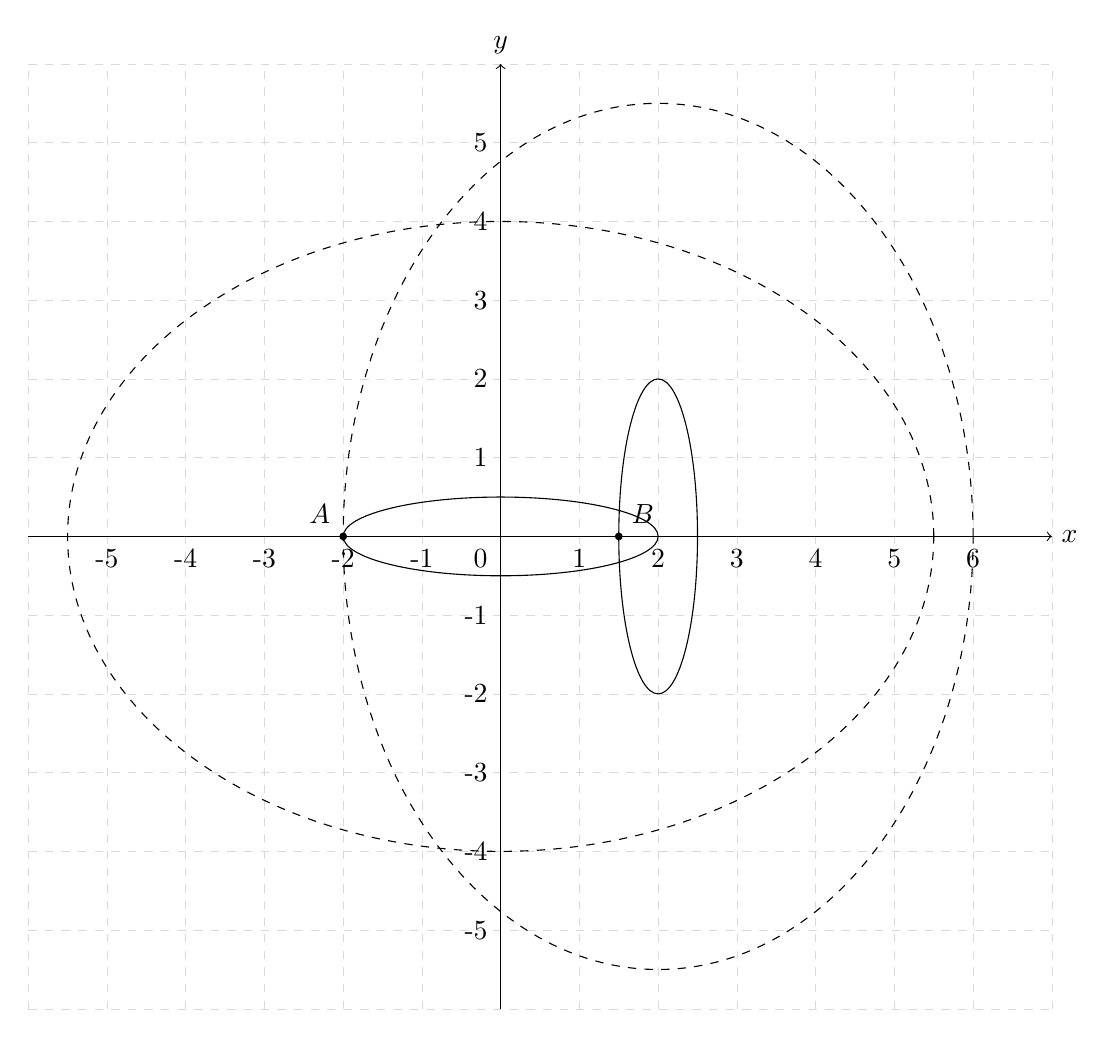
\begin{tikzpicture}
      \draw[help lines, color=gray!30, dashed] (-6,-6) grid (7,6);
      \draw[->] (-6,0)--(7,0) node[right]{$x$};
      \draw[->] (0,-6)--(0,6) node[above]{$y$};
      \node[inner sep=1pt,label=below left:{0}] at (0,0) {};
      \foreach \i in {-5,...,-1,1,2,3,4,5,6}
      {
        \node[inner sep=1pt,label=below:{\i}] at (\i,0) {};
      }
      \foreach \i in {-5,...,-1,1,2,3,4,5}
      {
        \node[inner sep=1pt,label=left:{\i}] at (0,\i) {};
      }
      \draw (0,0) ellipse (2 and 0.5);
      \draw (2,0) ellipse (0.5 and 2);
      \draw[dashed] (0,0) ellipse (5.5 and 4);
      \draw[dashed] (2,0) ellipse (4 and 5.5);
      \node[circle,inner sep=1pt,fill=black,label=above left:{$A$}] at (-2,0) {};
      \node[circle,inner sep=1pt,fill=black,label=above right:{$B$}] at (1.5,0) {};
    \end{tikzpicture}
  \caption{Эллипсы, между которыми ищем расстояние Хаусдорфа}
  \label{fig:hausdorff:example}
\end{figure}

Пунктиром нарисованы эллипсы $E + \varepsilon $ и $F + \varepsilon $ такие,
чтобы выполнялось \eqref{eq:hausdorff:distance}.
В данном случае $ \varepsilon $~---~это расстояние между точками $A$ и $B$,
которое равно $ \varepsilon = 1.5 - \left( -2 \right) = 3.5$.
Поэтому $H \left( E, D \right) = 3.5$.

\subsection{Пример 2}

Пусть $ \left( X, d \right) $~---~ метрическое пространство, $Y \subseteq X$ и $ \varepsilon > 0$.
Подмножество $S \subseteq X$ называется $ \varepsilon $-сетью для $Y$,
если для каждого $y \in Y$ найдётся такой $s \in S$, что $d \left( y, s \right) < \varepsilon $.
Если $Y = X$, то $S$ называется $ \varepsilon $-сетью в $X$.

Пусть $ \left( X, d \right) $~---~компактное метрическое пространство.
В $X$ возьмём конечную $ \varepsilon $-сеть.
Это значит, что
$ \left( \forall x \in X \right) \, \left( \exists s \in S \right) \, :
  \qquad d \left( x, s \right) < \varepsilon $.
Тогда расстояние Хаусдорфа между компактом $X$ и $ \varepsilon $-сетью равно
$H \left( X, S \right) = \varepsilon $.

\section{Случайные величины}

Имеем вероятностное пространство $ \left( \Omega, \mathcal{F}, \mathbb{P} \right) $,
где $ \Omega = \mathbb{R}^n, \, \mathcal{F} = \mathcal{B} \left( \mathbb{R}^n \right) $~---~
борелевская $ \sigma$-алгебра на $ \mathbb{R}^n, \, \mathbb{P}$~---~
вероятностная мера на $ \mathcal{F}$.

Есть два определения случайной величины:
\begin{enumerate}
  \item функция $ \xi \, : \, \Omega \to \mathbb{R}$ называется случайной величиной, если
  \begin{equation*}
    \forall \Delta \in \mathcal{B} \left( \mathbb{R} \right) \, : \qquad
    \xi^{-1} \left( \Delta \right) =
    \left\{ \omega \; \middle| \; \xi \left( \omega \right) \in \Delta \right\} \in \mathcal{F};
  \end{equation*}
  \item функция $ \xi \, : \, \Omega \to \mathbb{R}$ называется случайной величиной, если
  \begin{equation*}
    \forall c \in \mathbb{R} \, : \qquad
    \left\{ \omega \; \middle| \; \xi \left( \omega \right) \leq c \right\} =
    \xi^{-1} \left( \left( -\infty, c \right] \right) \in \mathcal{F}.
  \end{equation*}
\end{enumerate}

Проверим,
является ли расстояние Хаусдорфа
\begin{equation*}
  \gamma =
  H \left( AE + \vec{b} + \vec{ \xi }, F \right) =
  H \left( \xi \left( E \right), F \right)
\end{equation*}
случайной величиной, где $ \xi $~---~
случайное отображение из $ \mathbb{R}^n$ в $ \mathbb{R}^n$.

По определению \eqref{eq:hausdorff:distance}
\begin{gather*}
  \gamma =
  \inf \left\{
    \varepsilon \geq 0 \; \middle| \;
    \xi \left( E \right) + \varepsilon \subset F, \,
    F + \varepsilon \subset \xi \left( E \right) \right\} = \\
  = \inf \left\{
    \varepsilon \geq 0 \; \middle| \;
    \bigcup \limits_{x \in \xi \left( E \right) }
      \overline{B}_{ \varepsilon } \left( x \right) \subset F, \,
    \bigcup \limits_{x \in F} \overline{B}_{ \varepsilon }
      \left( x \right) \subset \xi \left( E \right)
  \right\}.
\end{gather*}

Чтобы это проверить, нужно выяснить, является ли случайной величиной число $ \varepsilon_n > 0$.
Если получится, то
\begin{equation*}
  \forall c \in \mathbb{R}: \qquad
  \left\{ \omega \; \middle| \; \inf \limits_n \varepsilon_n \left( \omega \right) \leq c \right\} =
  \bigcup \limits_{n = 1}^{ \infty }
    \left\{ \omega \; \middle| \; \varepsilon_n \left( \omega \right) \leq c \right\}.
\end{equation*}
Каждое множество, которые стоит под знаком объединения по определению
принадлежит $ \sigma $-алгебре $ \mathcal{F}$,
и их счётное объединение принадлежит $ \sigma $-алгебре $ \mathcal{F}$,
так как она замкнута относительно счётной операции объединения.
